\documentclass[conference,a4paper]{IEEEtran}

% Escritura mejorada de fórmulas matemáticas
\usepackage{amsmath}

% Inserción de gráficos
\usepackage{graphicx}

% Escritura de pseudocódigo
\usepackage[kw]{pseudo}

% Escritura mejorada de tablas
\usepackage{booktabs}

% Escritura mejorada de citas bibliográficas
\usepackage{cite}

% Hipervínculos en el documento
\usepackage{hyperref}


% Macros traducidas
\def\contentsname{Índice general}
\def\listfigurename{Índice de figuras}
\def\listtablename{Índice de tablas}
\def\refname{Referencias}
\def\indexname{Índice alfabético}
\def\figurename{Fig.}
\def\tablename{TABLA}
\def\partname{Parte}
\def\appendixname{Apéndice}
\def\abstractname{Resumen}
% IEEE specific names
\def\IEEEkeywordsname{Palabras clave}
\def\IEEEproofname{Demostración}


\begin{document}

\title{Título del trabajo (elegir uno original)}

\author{
  \IEEEauthorblockN{Aitana Valera Prados}
  \IEEEauthorblockA{
    \textit{Dpto. Ciencias de la Computación e Inteligencia Artificial}\\
    \textit{Universidad de Sevilla}\\
    Sevilla, España\\}
    \href{mailto:aitvalpra@alum.us.es}{aitvalpra@alum.us.es}
  
  \and
  
  \IEEEauthorblockN{Miguel Ángel Martínez Fernández}
  \IEEEauthorblockA{
    \textit{Dpto. Ciencias de la Computación e Inteligencia Artificial}\\
    \textit{Universidad de Sevilla}\\
    Sevilla, España\\}
    \href{mailto:migmarfer@alum.us.es}{migmarfer@alum.us.es}
}

\maketitle


% Resumen

\begin{abstract}
  Este trabajo tiene como objetivo principal evaluar el impacto y la ganancia de rendimiento que aporta la integración de métricas relacionales basadas en topología de redes combinadas con las técnicas tradicionales de minería de texto para la tarea de clasificación automática de artículos científicos. Empleando el conocido conjunto de datos Cora, se modela la estructura de citas bibliográficas mediante un grafo dirigido y no dirigido, extrayendo características estructurales avanzadas como centralidades de grado, intermediación, cercanía, PageRank, coeficientes de clustering y pertenencia a comunidades mediante algoritmos de modularidad codiciosa. 
  
  Las conclusiones demuestran de manera sólida que los modelos de clasificación entrenados exclusivamente con la bolsa de palabras (Bag of Words) mitigan ciertas ambigüedades terminológicas cuando se complementan con métricas puramente relacionales. Los clasificadores experimentaron variaciones notables en sus puntuaciones de rendimiento, evidenciando que el entorno social y de citación de una publicación aporta un contexto semántico implícito que las palabras clave por sí solas no logran capturar formalmente.
\end{abstract}


% Palabras claves
\begin{IEEEkeywords}
  Inteligencia Artificial, Minería de Grafos, Clasificación de Texto, Redes de Citas, Dataset Cora, Aprendizaje Supervisado.
\end{IEEEkeywords}


\section{Introducción}

En esta sección se dedican varios párrafos para dar el contexto en el que se desarrolla el trabajo presentado. El aumento exponencial de manuscritos académicos publicados diariamente en repositorios abiertos hace que la indexación temática manual sea una tarea inviable en términos de tiempo y recursos. Tradicionalmente, el procesamiento de lenguaje natural (PLN) ha abordado este reto analizando los resúmenes o textos completos mediante vectores de frecuencias de términos. Sin embargo, este enfoque estático ignora una de las señales de información más ricas presentes en la literatura académica: el hipervínculo natural establecido mediante la red de referencias cruzadas y citas bibliográficas~\cite{b1}.

Después vienen un par de párrafos para dar un poco más de detalle sobre el trabajo realizado. El presente proyecto aborda directamente la clasificación multiclase de publicaciones científicas combinando dos dimensiones de características independientes. Por un lado, los atributos textuales binarios que capturan la presencia o ausencia de un vocabulario controlado; por otro lado, variables numéricas continuas y discretas que formalizan la importancia estructural del documento en su red de citación. Para ello, se emplea el clásico conjunto de datos analítico \emph{Cora Dataset}, el cual agrupa miles de publicaciones de ciencias de la computación dentro de siete categorías temáticas bien delimitadas. La solución se enfoca en someter los conjuntos de datos combinados y aislados a procesos exhaustivos de optimización de hiperparámetros mediante validación cruzada.

Finalmente, el último párrafo se dedica a comentar la estructura del documento por secciones, como el que sigue. La Sección~II expone los fundamentos matemáticos de las técnicas relacionales y los algoritmos clasificadores seleccionados; la Sección~III profundiza en el pipeline de ingeniería de características implantado y detalla la codificación lógica de datos; en la Sección~IV se desglosan los resultados empíricos y matrices comparativas de rendimiento; y finalmente, en la Sección~V se sintetizan las deducciones del estudio y se abren futuras líneas de investigación.


\section{Preliminares}

En esta sección se hace una breve introducción de las técnicas empleadas y también trabajos relacionados, si los hay.

\subsection{Métodos empleados}

Del dataset obtenemos dos tablas, 
\begin{itemize}
\item \textbf{cora.content}
Contiene una tabla con el id del paper, 1433 columnas que representan una palabra, con un 1 si aparecen en el paper y un 0 si no (en realidad al hacer el dateset se eliminó toda palabra que apareciera menos de 10 veces, además de conectores textuales \cite{yang2015network}.) y la última columna representa la clase a la que pertenece el paper.

\item \textbf{cora.cites}
Contiene una tabla con el id del paper citado y el id del paper que lo cita.
\end{itemize}

 A partir de estos datos modelamos el conjunto de papers como un grafo dirigido, donde cada vértice representa un paper y cada arista dirigida una cita. $G_d = (V, E_d)$ y un grafo no dirigido correspondiente $G = (V, E)$. 
Hemos decidido usar el grafo no dirigido porque la mayoría de las propiedades topológicas analizadas dependen de la conectividad general y del volumen total de enlaces entre las publicaciones, sin que la orientación del flujo de citas altere la pertenencia a un núcleo temático. No obstante, se ha decidido conservar la naturaleza del grafo para calcular \texttt{pagerank}, porque de tal modo que el artículo $A$ cite al artículo $B$ otorga relevancia a $B$, pero no viceversa, y para 
 la detección de \texttt{comunidades}, porque los nichos se delimitan de manera mucho más precisa si se respeta la direccionalidad original.


Los métodos implementados se clasifican en los siguientes bloques fundamentales:

\begin{itemize}
\item \textbf{Métricas Relacionales de Centralidad:} Permiten cuantificar la relevancia de un nodo basado en sus enlaces. Se calculan las centralidades de grado entrante y saliente, la intermediación (\emph{betweenness}), la cercanía (\emph{closeness}) 
\begin{equation}
  \label{eq:ejemplo}
  C_C(u) = \frac{|V_u| - 1}{|V| - 1} \frac{|V_u| - 1}{\sum_{v \in V_u} d(v, u)}
\end{equation}
el prestigio a través del algoritmo PageRank, cuya probabilidad de transición e importancia estructural se define formalmente como
\begin{equation}
  \label{eq:pagerank}
  PR(u) = \frac{1-\alpha}{|V|} + \alpha \sum_{v \in B_u} \frac{PR(v)}{L(v)}
\end{equation}
donde $\alpha$ representa el factor de amortiguación (fijado en $0.85$), $B_u$ es el conjunto de nodos que apuntan a $u$, y $L(v)$ es el grado de salida del nodo $v$. Asimismo, el grado de cohesión vecinal se cuantifica mediante el coeficiente de clustering local
\begin{equation}
  \label{eq:clustering}
  C(u) = \frac{2 \, |\{ (v, w) \in E : v, w \in N_u \}|}{k_u (k_u - 1)}
\end{equation}
donde $N_u$ representa el conjunto de vecinos inmediatos del nodo $u$ y $k_u$ denota su grado total, midiendo la proporción de aristas existentes entre sus vecinos respecto al total de conexiones posibles.
\item \textbf{Detección de Comunidades:} Agrupamiento no supervisado basado en la densidad de conexiones internas, empleando la optimización de la modularidad codiciosa (\emph{Greedy Modularity}).
\item \textbf{Algoritmos de Clasificación Supervisada:} Implementación de los clasificadores optimizados mediante búsquedas en rejilla (\emph{GridSearchCV}).
\end{itemize}

\subsection{Trabajo Relacionado}

 El análisis predictivo sobre el dataset Cora constituye un campo de pruebas estándar dentro del aprendizaje de máquinas en grafos. Los estudios pioneros se limitaban al uso de clasificadores de contenido textual lineal, evolucionando rápidamente hacia marcos híbridos que emplean caminatas aleatorias o algoritmos de propagación de etiquetas (\emph{Label Propagation})~\cite{b3}. En la actualidad, aunque las Redes Convolucionales de Grafos (GCN) lideran los rankings de precisión, el análisis pormenorizado mediante ingeniería de características explícitas sigue siendo crítico para garantizar la explicabilidad.


\section{Metodología}

En primer lugar, partiendo de los dos archivos : \texttt{cora.content}  y \texttt{cora.cites} se construye el grafo  con la librería \texttt{networkx}, y como se ha explicado anteriormente se convierte en un grafo no dirigido.
\\
Posteriormente calculamos los atributos \texttt{centralidad-grado-in, centralidad-grado-out, centralidad-intermediacion, centralidad-cercania, pagerank, clustering y comunidad} como candidatos a ser las métricas relacionales que estaremos estudiando.
\\
Determinamos si una métrica es útil:
\begin{enumerate}
\item \textit{Distribución de méticas por clase \figurename~\ref{fig:distrMetricas}:}  los papers de distintas clases deberán tener valores distintos en esa métrica.

\begin{figure}[htbp]
  \centering
  
  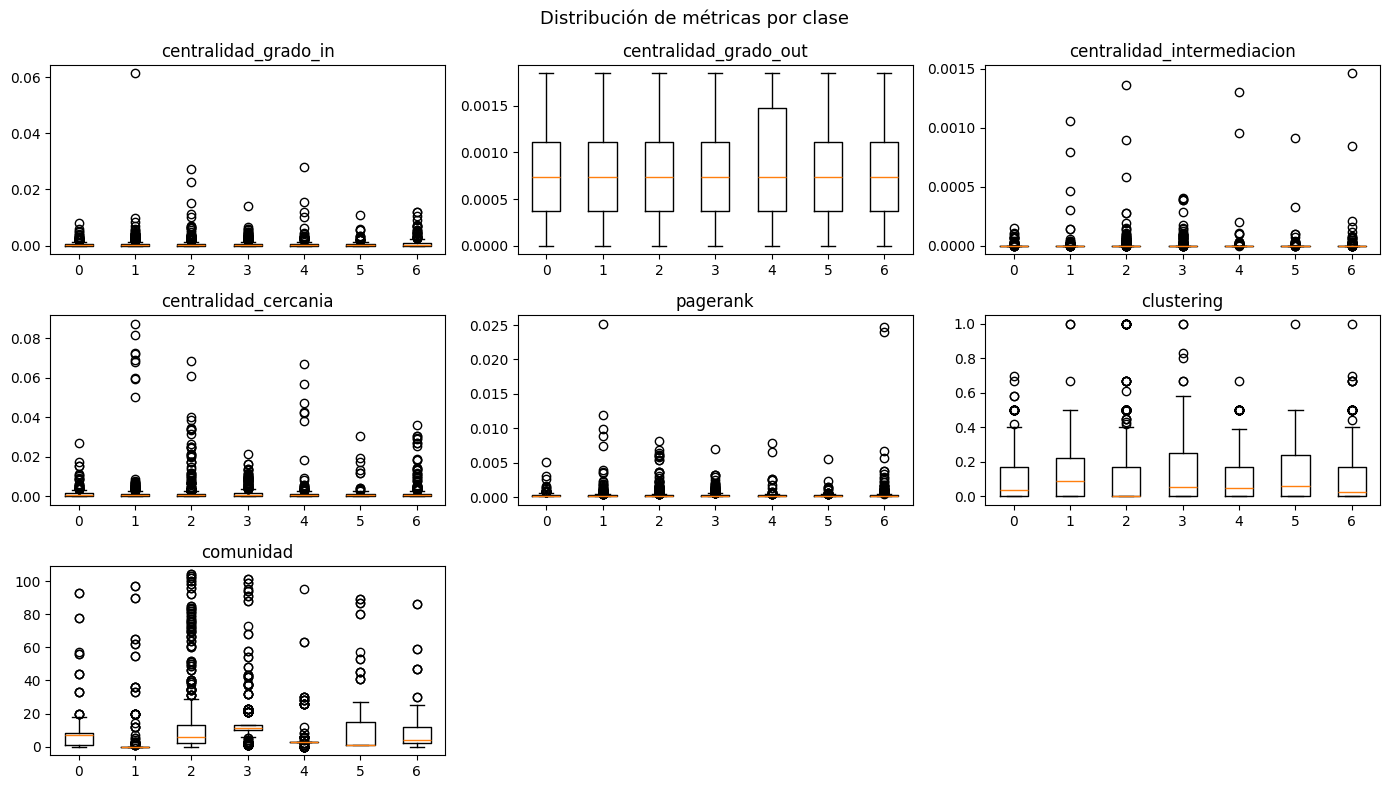
\includegraphics[width=0.45\textwidth]{dist-metricas-clase}
  \caption{Distribución de métricas por clase.}
  \label{fig:distrMetricas}
\end{figure}


\item\textit{Test de Kruskall-Wallis \tablename~\ref{tab:kruskall}:} El resultado produce un estadístico de prueba (llamado \(H\)) junto con un valor p (p-value) . \(p < 0.05\) determina que existen diferencias estadisticamente significativas entre, al menos, un par de grupos.

\begin{table}[htbp]
  \caption{Test de Kruskall-Wallis para métricas pre-seleccionadas}
  \label{tab:kruskall}
  \centering
  \begin{tabular}{lccc}
    \toprule
    Métrica Evaluada & H & p-value & ¿Pasa el test? \\
    \midrule
   \texttt{centralidad\_grado\_in}       & 6.45   & 0.3751 & No \\
    \texttt{centralidad\_grado\_out}      & 38.92  & 0.0000 & Sí \\
    \texttt{centralidad\_intermediacion}  & 9.89   & 0.1293 & No \\
    \texttt{centralidad\_cercania}        & 10.63  & 0.1006 & No \\
    \texttt{pagerank}                     & 6.92   & 0.3284 & No \\
    \texttt{clustering}                   & 27.26  & 0.0001 & Sí \\
    \texttt{comunidad}                    & 978.56 & 0.0000 & Sí \\
    
    \bottomrule
  \end{tabular}
\end{table}

 \item\textit{Correlación entre métricas \figurename~\ref{fig:corrleacionMetricas}:} Si la correlación entre dos atributos es muy alta (su valor absoluto es cercano a uno) podemos determinar que están midiendo lo mismo, pudiendo así eliminar uno de ellos.

\begin{figure}[htbp]
  \centering
  
  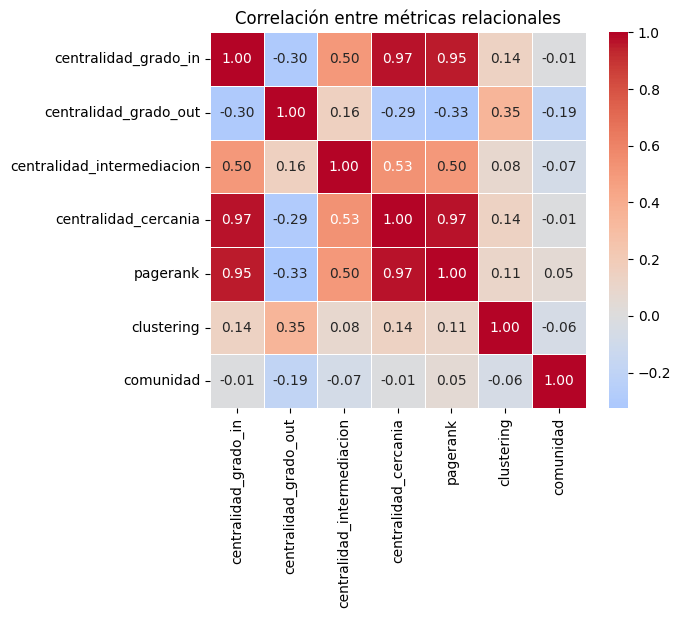
\includegraphics[width=0.45\textwidth]{Correlación entre métricas}
  \caption{Correlación entre métricas relacionales.}
  \label{fig:corrleacionMetricas}
\end{figure}

\end{enumerate}

Tras estas comprobaciones, nos quedamos con \texttt{centralidad-grado-out, clustering y comunidad} 

Ahora dividimos el conjunto en un 20\% para test el 80\% restante para entrenar los modelos, quedándonos con \texttt{2166} muestras de entrenamiento y \texttt{542} muestras de prueba.

Finalmente ejecutamos una búsqueda en rejilla, descrita en \figurename~\ref{pcd:rejilla} para cada modelo (como los resultados dependen de los hiperparámetros, estos últimos estarán definidos en el apartado de resultados).

\begin{figure}[htbp]
\footnotesize %
  \begin{pseudo}*
    \hd{\fn{busqueda\_en\_rejilla\_simple}}(X_{ent}, y_{ent}, X_{val}, y_{val}, \textnormal{rejilla}) \\*
    \multicolumn{2}{l}{\textbf{Entrada}: \parbox{0.38\textwidth}{Matrices de entrenamiento y validación con sus respectivos vectores objetivo.}} \\*
    \multicolumn{2}{l}{\textbf{Salida}: \parbox{0.38\textwidth}{El estimador optimizado con el mejor rendimiento obtenido.}} \\\( \textnormal{mejor\_puntuacion} \leftarrow -\infty \) \\
    \( p_{opt} \leftarrow \textnormal{nulo} \) \\
    \textbf{para cada} combinación de parámetros \( p \) \textbf{en} \textnormal{rejilla} \textbf{hacer} \\+
      Entrenar modelo con parámetros \( p \) usando \( X_{ent} \) y \( y_{ent} \) \\
      \( \textnormal{puntuacion} \leftarrow \textnormal{evaluar modelo en } X_{val} \textnormal{ e } y_{val} \) \\
      \textbf{si} \( \textnormal{puntuacion} > \textnormal{mejor\_puntuacion} \) \textbf{entonces} \\+
        \( \textnormal{mejor\_puntuacion} \leftarrow \textnormal{puntuacion} \) \\
        \( p_{opt} \leftarrow p \) \\--
   Entrenar estimador final con \( p_{opt} \) sobre \( X \) e \( y \) \\ %
    devolver estimador\_final
  \end{pseudo}
  \caption{Algoritmo general del pipeline de optimización GridSearch sin pliegues.}
  \label{pcd:rejilla}
\end{figure}


\section{Resultados}

Ahora detallaremos las pruebas realizadas, los datos y los resultados obtenidos:
\begin{itemize}
\item Los experimentos realizados dividieron los datos en un 80\% para entrenamiento y un 20\% para pruebas. Se configuró una búsqueda \texttt{GridSearchCV} para calibrar los parámetros clave de cada clasificador \\ 

\begin{enumerate}
\item \textbf{K-Nearest Neighbors (kNN):}
  \begin{itemize}
  \item Número de vecinos evaluados: $[1, 3, 5, 7, 9, 11, 13, 15]$.
  \item Funciones de distancia: Euclídea y Manhattan.
  \end{itemize}

\item \textbf{Árbol de Clasificación:}
  \begin{itemize}
  \item Profundidades máximas (\texttt{max\_depth}): Rango $[3, 11)$ (valores enteros del $3$ al $10$).
  \item Mínimo de muestras por hoja (\texttt{min\_samples\_leaf}): $[5, 10, 15]$.
  \end{itemize}

\item \textbf{Naive Bayes:}
  \begin{itemize}
  \item Parámetro de suavizado de Laplace (\texttt{alpha}): Rango $[1, 6)$ (valores enteros del $1$ al $5$).
  \item Transformador de discretización no lineal \texttt{KBinsDiscretizer(encode='ordinal', strategy='quantile')}.
  \end{itemize}
\end{enumerate}


\item Los resultados obtenidos se evaluaron utilizando la puntuación F1-macro para gestionar de manera justa el desbalance de clases nativo del conjunto Cora.
\item Análisis de los resultados: Para los 3 conjuntos de datos el modelo que mejor rendimiento ha obtenido ha sido el Árbol de decisión CART, con un F1-macro de 0,72 en el conjunto que incluye tanto las métricas relacionales como la bolsa de palabras. \\ 
La búsqueda en rejilla ha determinado que para este caso los mejores hiperparámetros son \texttt{max-depth= 9} y  \texttt{min-samples-leaf = 5}.
\end{itemize}


\begin{table}[htbp]
  \caption{Resultados Comparativos de Rendimiento para cada conjunto}
  \label{tab:ejemplo}
  \centering
  \begin{tabular}{lccc}
    \toprule
    Modelo Evaluado & Datos Totales & Solo BoW & Solo Relacionales \\
    \midrule
    CART		& \texttt{0,720} & \texttt{0,572} & \texttt{0,698} \\
    K-Nearest Neighbors & \texttt{0,414} & \texttt{0,413} & \texttt{0,514} \\
    Naive Bayes         & \texttt{0,388} & \texttt{0,066} & \texttt{0,388} \\
    
    \bottomrule
  \end{tabular}
\end{table}


\section{Conclusiones}

Finalmente, se dedica la última sección para indicar las conclusiones obtenidas del trabajo. La inclusión de variables topológicas aporta información complementaria valiosa, aunque su impacto final está condicionado por la naturaleza matemática del clasificador y la escala de las características continuas. 

Se suele dedicar un párrafo final con ideas de mejora y trabajo futuro. Como líneas de desarrollo futuro, se plantea la incorporación de esquemas de pesado TF-IDF, la normalización avanzada de las métricas estructurales mediante técnicas de escalado, o la exploración de modelos basados en ensamblados como XGBoost para optimizar las fronteras de decisión mixtas.


\begin{thebibliography}{00}
\bibitem{yang2015network}
C.~Yang, Z.~Liu, D.~Zhao, M.~Sun, y E.~Y. Chang, 
``Network Representation Learning with Rich Text Information,'' 
en \emph{Proceedings of the 24th International Joint Conference on Artificial Intelligence (IJCAI)}, 
2015, pp. 2111--2117.
\bibitem{b2} L. Page, S. Brin, R. Motwani, and T. Winograd, ``The PageRank citation ranking: Bringing order to the web,'' Stanford InfoLab, Tech. Rep., 1999.
\bibitem{b3} M. Sen, G. Namata, M. Bilgic, L. Getoor, B. Gallagher, and T. Eliassi-Rad, ``Collective classification in network data,'' AI Magazine, vol. 29, no. 3, pp. 93--106, 2008.
\end{thebibliography}

\end{document}
